% Generated by pysimcount.pfseeds -- do not edit; regenerate instead.
% figure: A-measured-by-order -- Suzuki formulas of each order, r from: Measured $r$; median over seeds [1, 2, 3, 4, 5, 6, 7, 8, 9, 10], bars = min..max
% metric=t gatebase=ct merged
% seed 1: git_commit=01d3c275ceae2840002bd1aaea68f59b987c4975 git_dirty=False
% seed 2: git_commit=01d3c275ceae2840002bd1aaea68f59b987c4975 git_dirty=False
% seed 3: git_commit=01d3c275ceae2840002bd1aaea68f59b987c4975 git_dirty=False
% seed 4: git_commit=01d3c275ceae2840002bd1aaea68f59b987c4975 git_dirty=False
% seed 5: git_commit=01d3c275ceae2840002bd1aaea68f59b987c4975 git_dirty=False
% seed 6: git_commit=01d3c275ceae2840002bd1aaea68f59b987c4975 git_dirty=False
% seed 7: git_commit=01d3c275ceae2840002bd1aaea68f59b987c4975 git_dirty=False
% seed 8: git_commit=01d3c275ceae2840002bd1aaea68f59b987c4975 git_dirty=False
% seed 9: git_commit=01d3c275ceae2840002bd1aaea68f59b987c4975 git_dirty=False
% seed 10: git_commit=01d3c275ceae2840002bd1aaea68f59b987c4975 git_dirty=False
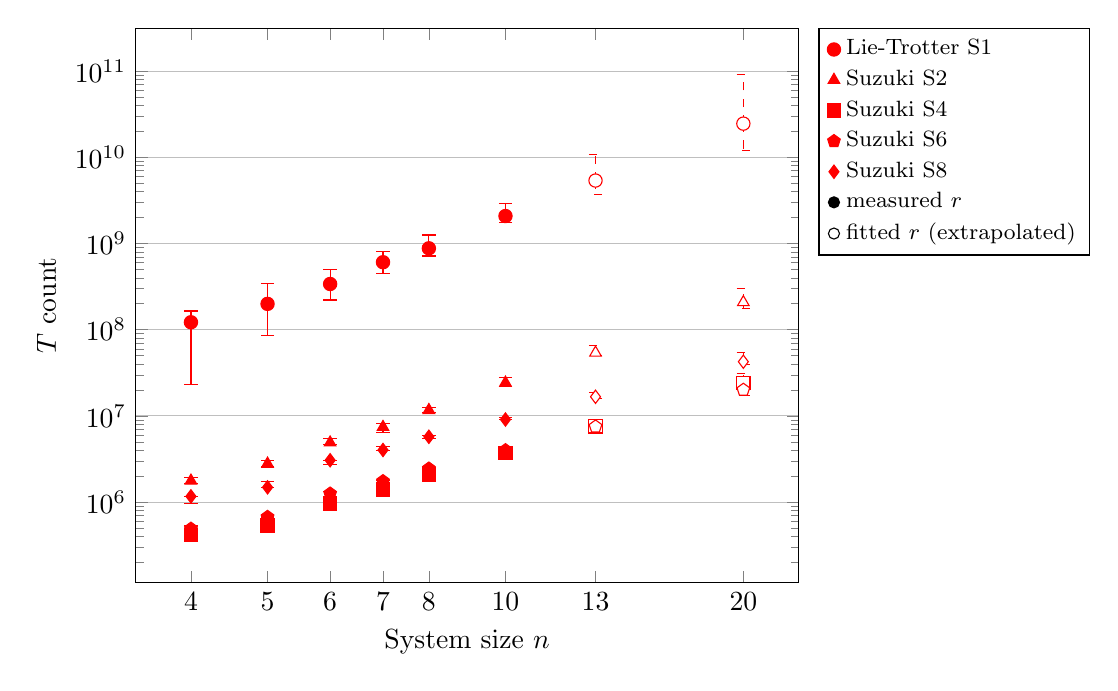
\begin{tikzpicture}
  \begin{loglogaxis}[
    width=10cm,
    xlabel={System size $n$},
    ylabel={$T$ count},
    xtick={4,5,6,7,8,10,13,20},
    xticklabels={4,5,6,7,8,10,13,20},
    ymajorgrids=true,
    legend pos=outer north east,
    legend cell align=left,
    legend style={font=\footnotesize},
  ]
    \addplot[only marks, red, mark=*, mark size=2.4pt, mark options={solid, fill=red}, error bars/.cd, y dir=both, y explicit, error bar style={red}] coordinates {
      (4,122032132) += (0,43012412) -= (0,98964458)
      (5,199402167) += (0,141546483) -= (0,114415587)
      (6,339047007) += (0,166002525) -= (0,117870207)
      (7,606237382) += (0,204620666) -= (0,155004910)
      (8,879209894) += (0,377799882) -= (0,162092340)
      (10,2082317356) += (0,862076772) -= (0,344145796)
    };
    \addlegendentry{Lie-Trotter S1}
    \addplot[only marks, red, mark=*, mark size=2.4pt, mark options={solid, fill=white}, forget plot, error bars/.cd, y dir=both, y explicit, error bar style={red, dashed}] coordinates {
      (13,5375044845) += (0,5310027219) -= (0,1702392705)
      (20,24572872883) += (0,66858476181) -= (0,12697597343)
    };
    \addplot[only marks, red, mark=triangle*, mark size=2.4pt, mark options={solid, fill=red}, error bars/.cd, y dir=both, y explicit, error bar style={red}] coordinates {
      (4,1770918) += (0,147882) -= (0,145186)
      (5,2788988) += (0,226588) -= (0,232918)
      (6,4900920) += (0,623180) -= (0,259036)
      (7,7419156) += (0,797708) -= (0,1059272)
      (8,11673189) += (0,947219) -= (0,761365)
      (10,24258489) += (0,3492291) -= (0,2298411)
    };
    \addlegendentry{Suzuki S2}
    \addplot[only marks, red, mark=triangle*, mark size=2.4pt, mark options={solid, fill=white}, forget plot, error bars/.cd, y dir=both, y explicit, error bar style={red, dashed}] coordinates {
      (13,54054476) += (0,12119840) -= (0,4232192)
      (20,208003079) += (0,94302923) -= (0,31889559)
    };
    \addplot[only marks, red, mark=square*, mark size=2.4pt, mark options={solid, fill=red}, error bars/.cd, y dir=both, y explicit, error bar style={red}] coordinates {
      (4,412976) += (0,1636) -= (0,14760)
      (5,535040) += (0,32200) -= (0,18800)
      (6,944950) += (0,72670) -= (0,49600)
      (7,1401914) += (0,62182) -= (0,84474)
      (8,2059726) += (0,70194) -= (0,107298)
      (10,3733848) += (0,423458) -= (0,39068)
    };
    \addlegendentry{Suzuki S4}
    \addplot[only marks, red, mark=square*, mark size=2.4pt, mark options={solid, fill=white}, forget plot, error bars/.cd, y dir=both, y explicit, error bar style={red, dashed}] coordinates {
      (13,7564669) += (0,1247087) -= (0,436653)
      (20,24179760) += (0,6979914) -= (0,2903274)
    };
    \addplot[only marks, red, mark=pentagon*, mark size=2.4pt, mark options={solid, fill=red}, error bars/.cd, y dir=both, y explicit, error bar style={red}] coordinates {
      (4,490685) += (0,40671) -= (0,1131)
      (5,672686) += (0,38464) -= (0,1442)
      (6,1254729) += (0,64127) -= (0,81529)
      (7,1747975) += (0,52889) -= (0,148923)
      (8,2446500) += (0,93082) -= (0,3420)
      (10,3997843) += (0,318145) -= (0,196833)
    };
    \addlegendentry{Suzuki S6}
    \addplot[only marks, red, mark=pentagon*, mark size=2.4pt, mark options={solid, fill=white}, forget plot, error bars/.cd, y dir=both, y explicit, error bar style={red, dashed}] coordinates {
      (13,7514691) += (0,974349) -= (0,801299)
      (20,20063997) += (0,4611641) -= (0,2718045)
    };
    \addplot[only marks, red, mark=diamond*, mark size=2.4pt, mark options={solid, fill=red}, error bars/.cd, y dir=both, y explicit, error bar style={red}] coordinates {
      (4,1166916) += (0,3384) -= (0,192396)
      (5,1485150) += (0,266208) -= (0,2082)
      (6,3060110) += (0,6170) -= (0,317900)
      (7,4023349) += (0,360779) -= (0,14839)
      (8,5725226) += (0,217410) -= (0,217100)
      (10,9084018) += (0,580614) -= (0,10982)
    };
    \addlegendentry{Suzuki S8}
    \addplot[only marks, red, mark=diamond*, mark size=2.4pt, mark options={solid, fill=white}, forget plot, error bars/.cd, y dir=both, y explicit, error bar style={red, dashed}] coordinates {
      (13,16670469) += (0,2093523) -= (0,729797)
      (20,42551241) += (0,11351927) -= (0,3129601)
    };
    \addlegendimage{only marks, black, mark=*}
    \addlegendentry{measured $r$}
    \addlegendimage{only marks, black, mark=*, mark options={fill=white}}
    \addlegendentry{fitted $r$ (extrapolated)}
  \end{loglogaxis}
\end{tikzpicture}
